\documentclass[]{article}
\usepackage{lmodern}
\usepackage{graphicx}
\usepackage{adjustbox}
\usepackage{amssymb,amsmath}
\usepackage{ifxetex,ifluatex}
\usepackage{listings}
\usepackage[T1]{fontenc}
\usepackage[utf8]{inputenc}
\usepackage{microtype}
\usepackage[margin=1in]{geometry}
\usepackage{hyperref}
\usepackage{framed}
\usepackage{graphicx,grffile}
\usepackage{fancyvrb}
\usepackage{multirow}
\makeatletter
\def\maxwidth{\ifdim\Gin@nat@width>\linewidth\linewidth\else\Gin@nat@width\fi}
\def\maxheight{\ifdim\Gin@nat@height>\textheight\textheight\else\Gin@nat@height\fi}
\makeatother
% Scale images if necessary, so that they will not overflow the page
% margins by default, and it is still possible to overwrite the defaults
% using explicit options in \includegraphics[width, height, ...]{}
\setkeys{Gin}{width=\maxwidth,height=\maxheight,keepaspectratio}
\setlength{\parindent}{0pt}
\setlength{\parskip}{6pt plus 2pt minus 1pt}
\setlength{\emergencystretch}{3em}  % prevent overfull lines
\providecommand{\tightlist}{%
  \setlength{\itemsep}{0pt}\setlength{\parskip}{0pt}}

%%% Change title format to be more compact
\usepackage{titling}

% Create subtitle command for use in maketitle
\newcommand{\subtitle}[1]{
  \posttitle{
    \begin{center}\large#1\end{center}
    }
}

\setlength{\droptitle}{-2em}
  \title{MSAN 604 - Homework 1}
  \pretitle{\vspace{\droptitle}\centering\huge}
  \posttitle{\par}
  \author{Andre Guimaraes Duarte}
  \preauthor{\centering\large\emph}
  \postauthor{\par}
  \predate{\centering\large\emph}
  \postdate{\par}
  \date{November 3, 2016}
  
% Redefines (sub)paragraphs to behave more like section*s
\ifx\paragraph\undefined\else
\let\oldparagraph\paragraph
\renewcommand{\paragraph}[1]{\oldparagraph{#1}\mbox{}}
\fi
\ifx\subparagraph\undefined\else
\let\oldsubparagraph\subparagraph
\renewcommand{\subparagraph}[1]{\oldsubparagraph{#1}\mbox{}}
\fi

\usepackage{color}

%%%%%%%%%%%%%%%%%%%%%%%%%%%%%%%%%%%%%%%%%%%%%%%%%%%%%%%%%%%%%%%%%%%%%%%%%%%%%%%%%%%%%%%%%%%%%%%%%%%%%%%%%%%%%%%%%%%%%%%
\begin{document}
\maketitle

\section{Textbook Problems}
\paragraph{1.1}
Let X and Y be two random variables with $E(Y) = \mu$ and $E(Y^2) < \infty$.

a. Show that the constant $c$ that minimizes $E[(Y - c)^2]$ is $c = \mu$.

\color{blue}
$E[(Y-c)^2] = E[(Y-c)(Y-c)]
            = E[Y^2 - 2cY + c^2]
            = E[Y^2] - 2cE[Y] + E[c^2]
            = E[Y^2] - 2c\mu + c^2$.

We solve $\frac{d E[(Y-c)^2]}{d c} = 0 \Leftrightarrow 2c - 2\mu = 0 \Leftrightarrow c = \mu$.

In addition, $\frac{d^2 E[(Y-c)^2]}{d c^2} = 2 > 0$, so it is a minimum.

Thus, the constant that minimizes $E[(Y - c)^2]$ is $c = \mu$.
\color{black}

b. Deduce that the random variable $f(X)$ that minimizes $E[(Y - f(X))^2|X]$ is $f(X) = E[Y|X]$.

\color{blue}
$E[(Y - f(X))^2|X] = E[Y^2 - 2Yf(X) + f^2(X)|X]
                   = E[Y^2|X] - 2E[Yf(X)|X] + E[f^2(X)|X]$.

$f^2(X)$ given $X$ is a constant, so we get:

$E[(Y - f(X))^2|X] = E[Y^2|X] - 2f(X)E[Y|X] + f^2(X)$.

From a), by taking $f(X) = c$ and $E[Y|X] = \mu$, we get that the random variable that minimizes $E[(Y - f(X))^2|X]$ is $f(X) = E[Y|X]$.
\color{black}

c. Deduce that the random variable $f(X)$ that minimizes $E[(Y - f(X))^2]$ is also $f(X) = E[Y|X]$.

\color{blue}
$E[(Y - f(X))^2] = E[E[(Y - f(X))^2|X]]$.

Therefore, from b), we can deduce that the random variable that minimizes $E[(Y - f(X))^2]$ is also $f(X) = E[Y|X]$.
\color{black}


\paragraph{1.3}
Show that a strictly stationary process with $E(X_i^2) < \infty$ is weakly stationary.

\color{blue}
Since the process is scritcly stationary, the joint distribution of $X_{t_1}, X_{t_2}, \ldots, X_{t_n}$ is the same as that of $X_{t_1+h}, X_{t_2+h}, \ldots, X_{t_n+h}$ for all $n, h, t_1, t_2, \ldots, t_n \in N$. In particular, this is true for $n=1$. Therefore, all $X_t$ have the same probability distribution. Therefore, we have:

\begin{itemize}
\item $E[X_i] = E[X_j]$ $\forall i, j$. So $E[X_i] = \mu_X$ is independent of $t$.
\item $E[X_i^2] = \sigma^2 < \infty$ (given)
\item $Cov(X_t, X_{t+h}) = E[X_tX_{t+h}] - E[X_t]E[X_{t+h}] = E[X_t^2] - E[X_t]^2 = \sigma^2 - \mu_X^2$ is independent of $t$.
\end{itemize}
$\therefore$ a strictly stationary process with $E(X_i^2) < \infty$ is weakly stationary.
\color{black}

\paragraph{1.4}
Let $\{Z_t\}$ be a sequence of independent normal random variables, each with mean $0$ and variance $\sigma^2$ , and let $a$, $b$, and $c$ be constants. Which, if any, of the following processes are stationary? For each stationary process specify the mean and autocovariance function.

a. $X_t = a + bZ_t + cZ_{t-2}$

\color{blue}
\begin{itemize}
\item $\mu_X(t) = E[a + bZ_t + cZ_{t-2}]
                = E[a] + bE[Z_t] + cE[Z_{t-2}]
                = a$
\item 
\begin{tabular}{ccl}
$\gamma_X(t, t+h)$ & = & $Cov(X_t, X_{t+h})$\\
                  & = & $Cov(a + bZ_t + cZ_{t-2}, a + bZ_{t+h} + cZ_{t+h-2})$\\
                  & = & $Cov(a, a) + Cov(a, bZ_{t+h}) + Cov(a, cZ_{t+h-2}) +$\\
                  &   & $Cov(bZ_t, a) + Cov(bZ_t, bZ_{t+h}) + Cov(bZ_t, cZ_{t+h-2}) +$\\
                  &   & $Cov(cZ_{t-2}, a) + Cov(cZ_{t-2}, bZ_{t+h}) + Cov(cZ_{t-2}, cZ_{t+h-2})$\\
                  & = & $b^2Cov(Z_t, Z_{t+h}) + bcCov(Z_t, Z_{t+h-2}) + cbCov(Z_{t-2}, Z_{t+h}) + c^2Cov(Z_{t-2}, Z_{t+h-2})$\\
                  & = & $\begin{cases} (b^2 + c^2)\sigma^2 & \mbox{if } h=0\\ bc\sigma^2 & \mbox{if } h \pm 2\\ 0 & \mbox{otherwise} \end{cases}$\\
\end{tabular}
\end{itemize}
$\mu_X(t)$ and $\gamma_X(t, t+h)$ are independent of $t$, so the process is weakly stationary.
\color{black}

b. $X_t = Z_1 cos(ct) + Z_2 sin(ct)$

\color{blue}
\begin{itemize}
\item $\mu_X(t) = E[Z_1 cos(ct) + Z_2 sin(ct)]
                = E[z_1]cos(ct) + E[Z_2]sin(ct)
                = 0 + 0
                = 0$
\item
\begin{tabular}{ccl}
$\gamma_X(t, t+h)$ & = & $Cov(X_t, X_{t+h})$\\
                  & = & $Cov(Z_1 cos(ct) + Z_2 sin(ct), Z_1 cos(c(t+h)) + Z_2 sin(c(t+h)))$\\
                  & = & $Cov(Z_1 cos(ct), Z_1 cos(c(t+h))) + Cov(Z_1 cos(ct), Z_2 sin(c(t+h))) +$\\
                  &   & $Cov(Z_2 sin(ct), Z_1 cos(c(t+h))) + Cov(Z_2 sin(ct), Z_2 sin(c(t+h)))$\\
                  & = & $cos(ct) cos(c(t+h)) Cov(Z_1, Z_1) + cos(ct) sin(c(t+h)) Cov(Z_1, Z_2) +$\\
                  &   & $sin(ct) cos(c(t+h)) Cov(Z_2, Z_1) + sin(ct) sin(c(t+h)) Cov(Z_2, Z_2)$\\
                  & = & $\sigma^2 (cos(ct) cos(c(t+h)) + sin(ct) sin(c(t+h)))$\\
                  & = & $\sigma^2 cos(ct - c(t+h))$\\
                  & = & $\sigma^2 cos(ch)$\\
\end{tabular}
\end{itemize}
$\mu_X(t)$ and $\gamma_X(t, t+h)$ are independent of $t$, so the process is weakly stationary.
\color{black}

c. $X_t = Z_t cos(ct) + Z_{t-1} sin(ct)$

\color{blue}
\begin{itemize}
\item $\mu_X(t) = E[Z_t cos(ct) + Z_{t-1} sin(ct)]
                = E[Z_t cos(ct)] + E[Z_{t-1} sin(ct)]
                = E[Z_t] cos(ct) + E[Z_{t-1}] sin(ct)
                = 0 + 0
                = 0$
\item
\begin{tabular}{ccl}
$\gamma_X(t, t+h)$ & = & $Cov(X_t, X_{t+h})$\\
                  & = & $Cov(Z_t cos(ct) + Z_{t-1} sin(ct), Z_{t+h} cos(c(t+h)) + Z_{t+h-1} sin(c(t+h)))$\\
                  & = & $Cov(Z_t cos(ct), Z_{t+h} cos(c(t+h))) + Cov(Z_t cos(ct), Z_{t+h-1} sin(c(t+h))) +$\\
                  &   & $Cov(Z_{t-1} sin(ct), Z_{t+h} cos(c(t+h))) + Cov(Z_{t-1} sin(ct), Z_{t+h-1} sin(c(t+h)))$\\
                  & = & $cos(ct) cos(c(t+h)) Cov(Z_t, Z_{t+h}) + cos(ct) sin(c(t+h)) Cov(Z_t, Z_{t+h-1}) +$\\
                  &   & $sin(ct) cos(c(t+h)) Cov(Z_{t-1}, Z_{t+h}) + sin(ct) sin(c(t+h)) Cov(Z_{t-1}, Z_{t+h-1})$\\
                  & = & $\begin{cases} \sigma^2 & \mbox{if } h=0\\ \sigma^2 cos(ct) sin(c(t+1)) & \mbox{if } h = 1\\ \sigma^2 sin(ct) cos(c(t-1)) & \mbox{if } h = -1 \\ 0 & \mbox{otherwise} \end{cases}$\\
\end{tabular}
\end{itemize}
$\mu_X(t)$ is independent of $t$. $\gamma_X(t, t+h)$ is independent of $t$ only when $c = \pm k\pi$, where $k \in Z$. The process is therefore weakly stationary only when this condition is satisfied.
\color{black}

d. $X_t = a + bZ_0$

\color{blue}
\begin{itemize}
\item $\mu_X(t) = E[a + bZ_0]
                = E[a] + E[bZ_0]
                = a$
\item 
\begin{tabular}{ccl}
$\gamma_X(t, t+h)$ & = & $Cov(X_t, X_{t+h})$\\
                  & = & $Cov(a + bZ_0, a + bZ_0)$\\
                  & = & $Cov(a, a) + Cov(a, bZ_0) + Cov(bZ_0, a) + Cov(bZ_0, bZ_0)$\\
                  & = & $b^2Cov(Z_0, Z_0)$\\
                  & = & $\sigma^2 b^2$\\
\end{tabular}
\end{itemize}
$\mu_X(t)$ and $\gamma_X(t, t+h)$ are independent of $t$, so the process is weakly stationary.
\color{black}

e. $X_t = Z_0 cos(ct)$

\color{blue}
\begin{itemize}
\item $\mu_X(t) = E[Z_0 cos(ct)]
                = E[Z_0] cos(ct)
                = 0$
\item 
\begin{tabular}{ccl}
$\gamma_X(t, t+h)$ & = & $Cov(X_t, X_{t+h})$\\
                  & = & $Cov(Z_0 cos(ct), Z_0 cos(c(t+h)))$\\
                  & = & $cos(ct) cos(c(t+h)) Cov(Z_0, Z_0)$\\
                  & = & $cos(ct) cos(c(t+h)) \sigma^2$\\
\end{tabular}
\end{itemize}
$\mu_X(t)$ is independent of $t$. $\gamma_X(t, t+h)$ is independent of $t$ only when $c = \pm k\pi$, where $k \in Z$. The process is therefore weakly stationary only when this condition is satisfied.
\color{black}

f. $X_t = Z_t Z_{t-1}$

\color{blue}
\begin{itemize}
\item $\mu_X(t) = E[Z_t Z_{t-1}]
                = 0$
\item 
\begin{tabular}{ccl}
$\gamma_X(t, t+h)$ & = & $Cov(X_t, X_{t+h})$\\
                  & = & $Cov(Z_t Z_{t-1}, Z_{t+h} Z_{t+h-1})$\\
                  & = & $E[Z_t Z_{t-1} Z_{t+h} Z_{t+h-1}]$\\
                  & = & $\begin{cases} \sigma^4 & \mbox{if } h=0\\ 0 & \mbox{otherwise} \end{cases}$\\
\end{tabular}
\end{itemize}
$\mu_X(t)$ and $\gamma_X(t, t+h)$ are independent of $t$, so the process is weakly stationary.
\color{black}


\paragraph{1.7}
If $\{X_t\}$ and $\{Y_t\}$ are uncorrelated stationary sequences, i.e., if $X_r$ and $Y_s$ are uncorrelated for every $r$ and $s$, show that $\{X_t + Y_t\}$ is stationary with autocovariance function equal to the sum of the autocovariance functions of $\{X_t\}$ and $\{Y_t\}$ .

\color{blue}
$\mu_{X+Y} = E[X_t + Y_t]
           = E[X_t] + E[Y_t]
           = \mu_X + \mu_Y$

$\gamma_{X+Y}(h) = Cov(X_t + Y_t, X_{t+h} + Y_{t+h}) = Cov(X_t, X_{t+h}) + Cov(Y_t, Y_{t+h}) = \gamma_X(h) + \gamma_Y(h)$

$\mu_{X+Y}$ and $\gamma_{X+Y}(h)$ are independent of $t$, so the process is stationary.
\color{black}

\paragraph{2.3}
a. Find the ACVF of the time series $X_t = Z_t + .3 Z_{t-1} - .4 Z_{t-2}$ , where ${Z_t} \sim WN(0, 1)$.

\color{blue}
$E[X_t] = E[Z_t + .3 Z_{t-1} - .4 Z_{t-2}]
        = E[Z_t] + .3E[Z_{t-1}] - .4E[Z_{t-2}]
        = 0$

\begin{tabular}{ccl}
$\gamma_X(h)$ & = & $Cov(X_t, X_{t+h})$\\
              & = & $Cov(Z_t + .3 Z_{t-1} - .4 Z_{t-2}, Z_{t+h} + .3 Z_{t+h-1} - .4 Z_{t+h-2})$\\
              & = & $Cov(Z_t, Z_{t+h}) + Cov(Z_t, .3 Z_{t+h-1}) + Cov(Z_t, - .4 Z_{t+h-2}) +$\\
              &   & $Cov(.3 Z_{t-1}, Z_{t+h}) + Cov(.3 Z_{t-1}, .3 Z_{t+h-1}) + Cov(.3 Z_{t-1}, - .4 Z_{t+h-2}) +$\\
              &   & $Cov(- .4 Z_{t-2}, Z_{t+h}) + Cov(- .4 Z_{t-2}, .3 Z_{t+h-1}) + Cov(- .4 Z_{t-2}, - .4 Z_{t+h-2})$\\
              & = & $Cov(Z_t, Z_{t+h}) + .3Cov(Z_t, Z_{t+h-1}) - .4Cov(Z_t, Z_{t+h-2}) +$\\
              &   & $.3Cov(Z_{t-1}, Z_{t+h}) + .09Cov(Z_{t-1}, Z_{t+h-1}) - .12Cov(Z_{t-1},  Z_{t+h-2}) +$\\
              &   & $-.4Cov(Z_{t-2}, Z_{t+h}) - .12Cov(Z_{t-2}, Z_{t+h-1}) + .16Cov(Z_{t-2}, Z_{t+h-2})$\\
              & = & 
$\begin{cases}
-.4 & \mbox{if } h=-2\\
.3-.12 = .18 & \mbox{if } h=-1\\
1+.09+.16 = 1.25 & \mbox{if } h=0\\
.3-.12 = .18 & \mbox{if } h=1\\
-.4 & \mbox{if } h=2\\
0 & \mbox{otherwise}
\end{cases}$\\
\end{tabular}
\color{black}

b. Find the ACVF of the time series $Y_t = \tilde{Z}_t - 1.2 \tilde{Z}_{t-1} - 1.6 \tilde{Z}_{t-2}$ , where ${\tilde{Z}_t} \sim WN(0, .25)$. Compare with the answer found in (a).

\color{blue}
$E[Y_t] = E[\tilde{Z}_t - 1.2 \tilde{Z}_{t-1} - 1.6 \tilde{Z}_{t-2}]
        = E[\tilde{Z}_t] - 1.2E[\tilde{Z}_{t-1}] - 1.6E[\tilde{Z}_{t-2}]
        = 0$

\begin{tabular}{ccl}
$\gamma_Y(h)$ & = & $Cov(Y_t, Y_{t+h})$\\
              & = & $Cov(\tilde{Z}_t - 1.2 \tilde{Z}_{t-1} - 1.6 \tilde{Z}_{t-2}, \tilde{Z}_{t+h} - 1.2 \tilde{Z}_{t+h-1} - 1.6 \tilde{Z}_{t+h-2})$\\
              & = & $Cov(\tilde{Z}_t, \tilde{Z}_{t+h}) + Cov(\tilde{Z}_t, - 1.2 \tilde{Z}_{t+h-1}) + Cov(\tilde{Z}_t, - 1.6 \tilde{Z}_{t+h-2}) +$\\
              &   & $Cov(- 1.2 \tilde{Z}_{t-1}, \tilde{Z}_{t+h}) + Cov(- 1.2 \tilde{Z}_{t-1}, - 1.2 \tilde{Z}_{t+h-1}) + Cov(- 1.2 \tilde{Z}_{t-1}, - 1.6 \tilde{Z}_{t+h-2}) +$\\
              &   & $Cov(- 1.6 \tilde{Z}_{t-2}, \tilde{Z}_{t+h}) + Cov(- 1.6 \tilde{Z}_{t-2}, - 1.2 \tilde{Z}_{t+h-1}) + Cov(- 1.6 \tilde{Z}_{t-2}, - 1.6 \tilde{Z}_{t+h-2})$\\
              & = & $Cov(\tilde{Z}_t, \tilde{Z}_{t+h}) - 1.2Cov(\tilde{Z}_t, \tilde{Z}_{t+h-1}) - 1.6Cov(\tilde{Z}_t, \tilde{Z}_{t+h-2}) +$\\
              &   & $-1.2Cov(\tilde{Z}_{t-1}, \tilde{Z}_{t+h}) + 1.44Cov(\tilde{Z}_{t-1}, \tilde{Z}_{t+h-1}) + 1.92Cov(\tilde{Z}_{t-1}, \tilde{Z}_{t+h-2}) +$\\
              &   & $-1.6Cov(\tilde{Z}_{t-2}, \tilde{Z}_{t+h}) + 1.92Cov(\tilde{Z}_{t-2}, \tilde{Z}_{t+h-1}) + 2.56Cov(\tilde{Z}_{t-2}, \tilde{Z}_{t+h-2})$\\
              & = & 
$\begin{cases}
.25(-1.6) = -.4 & \mbox{if } h=-2\\
.25(-1.2+1.92) = .18 & \mbox{if } h=-1\\
.25(1+1.44+2.56) = 1 & \mbox{if } h=0\\
.25(-1.2+1.92) = .18 & \mbox{if } h=1\\
.25(-1.6) = -.4 & \mbox{if } h=2\\
0 & \mbox{otherwise}
\end{cases}$\\
\end{tabular}

We can see that the results from a) and b) are identical. 
\color{black}


\section{Additional Problems}
\paragraph{1}
Consider an MA(q) process, for general q.

(a) Find the autocovariance function of $\{X_t\} \sim MA(q)$.

\color{blue}
$X_t = Z_t + \theta_1 Z_{t-1} + \theta_2 Z_{t-2} + \ldots + \theta_q Z_{t-q}$, where $\{Z_t\} \sim WN(0, \sigma^2)$ and $\theta_i$ for $i \in N$ are constants.

\begin{tabular}{ccl}
$E[X_t]$ & = & $E[Z_t + \theta_1 Z_{t-1} + \theta_2 Z_{t-2} + \ldots + \theta_q Z_{t-q}]$\\
         & = & $E[Z_t] + \theta_1 E[Z_{t-1}] + \theta_2 E[Z_{t-2}] + \ldots + \theta_q E[Z_{t-q}]$\\
         & = & 0\\
\end{tabular}

\begin{tabular}{ccl}
$\gamma_X(t)$ & = & $Cov(X_t, X_{t+h})$\\
              & = & $Cov(Z_t, Z_{t+h}) + \theta_1 Cov(Z_t, Z_{t+h-1}) + \theta_2 Cov(Z_t, Z_{t+h-2}) + \ldots$\\
              &   & $+ \theta_1 Cov(Z_{t-1}, Z_{t+h}) + \theta_1^2 Cov(Z_{t-1}, Z_{t+h-1}) + \theta_1 \theta_2 Cov(Z_{t-1}, Z_{t+h-2}) + \ldots$\\
              &   & $+ \theta_2 Cov(Z_{t-2}, Z_{t+h}) + \theta_2 \theta_1 Cov(Z_{t-2}, Z_{t+h-1}) + \theta_2^2 Cov(Z_{t-2}, Z_{t+h-2}) + \ldots$\\
              &   & $+ \ldots$\\
              & = &
$\begin{cases}
\sigma^2(1 + \theta_1^2 + \theta_2^2 + \ldots + \theta_q^2) & \mbox{if } h = 0\\
\sigma^2(\theta_1 + \theta_1 \theta_2 + \theta_2 \theta_3 + \ldots + \theta_{q-1} \theta_q) & \mbox{if } h \pm 1\\
\sigma^2(\theta_2 + \theta_2 \theta_3 + \theta_3 \theta_4 + \ldots + \theta_{q-1} \theta_q) & \mbox{if } h \pm 2\\
\ldots & \ldots\\
\sigma^2(\theta_{q-1} + \theta_{q-1} \theta_q) & \mbox{if } h \pm q-1\\
\sigma^2(\theta_q) & \mbox{if } h \pm q-1\\
0 & \mbox{otherwise}
\end{cases}$\\
\end{tabular}
\color{black}

(b) Find the autocorrelation function of $\{X_t\} \sim MA(q)$.

\color{blue}
From a), we get:

$\gamma_X(0) = \sigma^2(1 + \theta_1^2 + \theta_2^2 + \ldots + \theta_q^2)$

So we get:

\begin{tabular}{ccl}
$\rho_X(h)$ & = & $\frac{\gamma_X(h)}{\gamma_X(0)}$\\
            & = &
$\begin{cases}
1 & \mbox{if } h = 0\\
\frac{\theta_1 + \theta_1 \theta_2 + \theta_2 \theta_3 + \ldots + \theta_{q-1} \theta_q}{1 + \theta_1^2 + \theta_2^2 + \ldots + \theta_q^2} & \mbox{if } h \pm 1\\
\frac{\theta_2 + \theta_2 \theta_3 + \theta_3 \theta_4 + \ldots + \theta_{q-1} \theta_q}{1 + \theta_1^2 + \theta_2^2 + \ldots + \theta_q^2} & \mbox{if } h \pm 2\\
\ldots & \ldots\\
\frac{\theta_{q-1} + \theta_{q-1} \theta_q}{1 + \theta_1^2 + \theta_2^2 + \ldots + \theta_q^2} & \mbox{if } h \pm q-1\\
\frac{\theta_q}{1 + \theta_1^2 + \theta_2^2 + \ldots + \theta_q^2} & \mbox{if } h \pm q-1\\
0 & \mbox{otherwise}
\end{cases}$\\
\end{tabular}
\color{black}

(c) Using your answer in part (b), deduce that an MA(q) process is q-correlated.

\color{blue}
From the result obtained in b), we can see that $\rho_X(h)$ is zero for $|h| > q$ and not necessarily zero for $|h| \leq q$. Therefore, an MA(q) process is q-correlated.
\color{black}

\paragraph{2}
The file \texttt{SALES.txt} includes 12 years of monthly sales (in thousands of dollars) beginning from January 1999 for a company that produces an accounting software. Interest lies in modeling the data as a function of time and predicting the future sales. Use the following command lines to read the data into R and format it as a time series object:

\begin{Verbatim}[frame=single]
sales <- read.table('SALES.txt')
sales <- ts(sales, start=1999, frequency=12)
\end{Verbatim}

(a) Fit a “trend only” model to the data where the trend component is quadratic in time, and comment on the fit of the model. For full marks, you should fit the model (provide your commented R code along with the R output), and provide full residual diagnostics.

\color{blue}
We decide to fit a "trend only" model where the trend component is quadratic in time. The R code used for this is shown below:

\begin{Verbatim}[frame=single]
# Extracting time as the explanatory variate from the time series framework of data
t <- time(sales)

# model quadratic trend
quad <- lm(sales~t+I(t^2))
summary(quad)
plot(sales, ylab='Sales', main='Quadratic trends of monthly sales')
# superimpose the fit of model quad on the plot of the data
points(t,predict.lm(quad), type='l', col='red')
\end{Verbatim}

This produces the plot of fit shown in Figure \ref{quad}. This seems to adequately model the general trend of sales.

\begin{figure}[!ht]
\centering
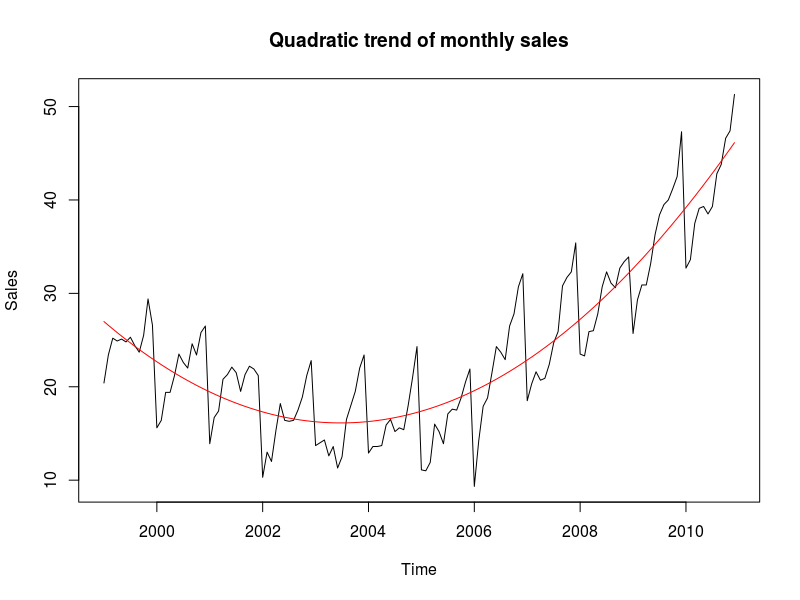
\includegraphics[width=\textwidth]{quad.png}
\caption{Plot of the fit for the quadratic trend model.}
\label{quad}
\end{figure}

Indeed, the output of \texttt{summary}, shown below, indicate that all predictor variables are significant, as well as the model in general. By using this model as is, an adjusted R-squared of $0.812$ is obtained, meaning that $81.2\%$ of the variability in prices is explained by the model.

\begin{verbatim}
Call:
lm(formula = sales ~ t + I(t^2))

Residuals:
     Min       1Q   Median       3Q      Max 
-10.2493  -2.7326  -0.2823   2.6100   9.5576 

Coefficients:
              Estimate Std. Error t value Pr(>|t|)    
(Intercept)  2.175e+06  1.211e+05   17.95   <2e-16 ***
t           -2.171e+03  1.208e+02  -17.97   <2e-16 ***
I(t^2)       5.419e-01  3.014e-02   17.98   <2e-16 ***
---
Signif. codes:  0 ‘***’ 0.001 ‘**’ 0.01 ‘*’ 0.05 ‘.’ 0.1 ‘ ’ 1

Residual standard error: 3.881 on 141 degrees of freedom
Multiple R-squared:  0.8146,  Adjusted R-squared:  0.812 
F-statistic: 309.8 on 2 and 141 DF,  p-value: < 2.2e-16
\end{verbatim}

In order to assess the model, we perform diagnostics on the residuals, as shown in Figure \ref{diag_quad}. 

\begin{figure}[!ht]
\centering
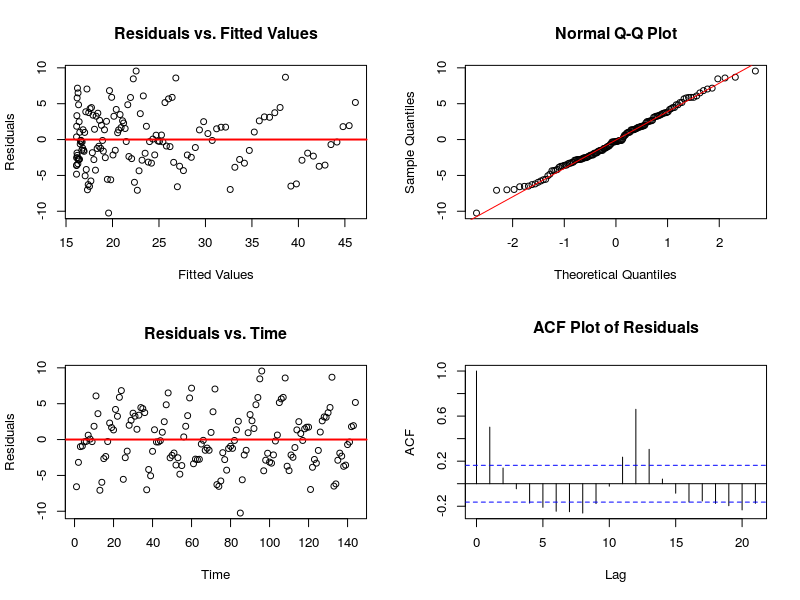
\includegraphics[width=\textwidth]{diag_quad.png}
\caption{Diagnostic plots for quadratic trend model.}
\label{diag_quad}
\end{figure}

We can see from the first plot that no "funnel-shape" is present, so we can say that the residuals are homoskedastic. The QQ-plot indicates that the residuals do not deviate too much from normality. From the sequence plot, we can say that the residuals seem independent. Finally, the ACF plot indicates that there is a seasonality effect in the data that has not been integrated in the current model.

\color{black}

(b) In accordance with a classical decomposition model, add a seasonal component to the quadratic regression model above, and comment on the fit of the model. Here, the seasonal component should capture the effect of month through the use of indicator variables. For full marks, you should fit the model (provide your commented R code along with the R output), and provide full residual diagnostics.

\color{blue}
In order to add a seasonal component to the quadratic regression model above, we use the following code:

\begin{Verbatim}[frame=single]
# Introducing month as the season
month <- as.factor(cycle(sales)) 

# model quadratic trend + seasonality
seas <- lm(sales~t+I(t^2)+month) 
summary(seas)
plot(sales, ylab='Sales', main='Quadratic and seasonal trends of monthly sales')
# superimpose the fit of model seas on the plot of the data
points(t,predict.lm(seas), type='l', col='red')
\end{Verbatim}

This produces the plot of fit shown in Figure \ref{seas}. The model seems to be doing a good job of modeling the pattern of sales in the data set.

\begin{figure}[!ht]
\centering
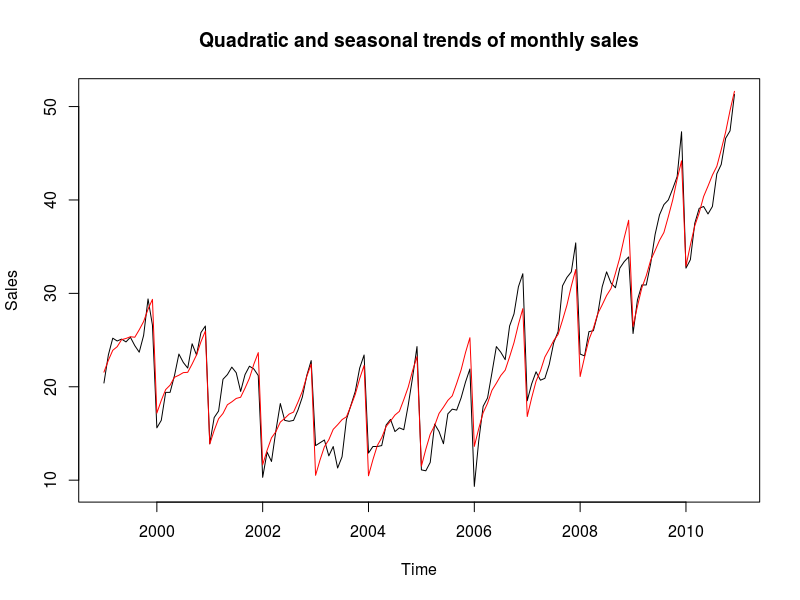
\includegraphics[width=\textwidth]{seas.png}
\caption{Plot of the fit for the quadratic trend and seasonality model.}
\label{seas}
\end{figure}

Indeed, the output of \texttt{summary}, shown below, indicate that all predictor variables are significant, as well as the model in general. By using this model, an adjusted R-squared of $0.948$ is obtained, meaning that $94.8\%$ of the variability in prices is explained by the model.

\begin{verbatim}
Call:
lm(formula = sales ~ t + I(t^2) + month)

Residuals:
    Min      1Q  Median      3Q     Max 
-4.6296 -1.3720  0.0598  1.2164  4.0276 

Coefficients:
              Estimate Std. Error t value Pr(>|t|)    
(Intercept)  2.175e+06  6.356e+04  34.219  < 2e-16 ***
t           -2.171e+03  6.340e+01 -34.243  < 2e-16 ***
I(t^2)       5.418e-01  1.581e-02  34.267  < 2e-16 ***
month2       1.674e+00  8.313e-01   2.014 0.046047 *  
month3       3.144e+00  8.313e-01   3.782 0.000236 ***
month4       3.922e+00  8.314e-01   4.718 6.06e-06 ***
month5       5.060e+00  8.315e-01   6.086 1.21e-08 ***
month6       5.565e+00  8.316e-01   6.693 5.93e-10 ***
month7       6.121e+00  8.317e-01   7.360 1.86e-11 ***
month8       6.428e+00  8.318e-01   7.728 2.61e-12 ***
month9       7.577e+00  8.319e-01   9.108 1.29e-15 ***
month10      8.811e+00  8.321e-01  10.589  < 2e-16 ***
month11      1.047e+01  8.323e-01  12.580  < 2e-16 ***
month12      1.186e+01  8.325e-01  14.240  < 2e-16 ***
---
Signif. codes:  0 ‘***’ 0.001 ‘**’ 0.01 ‘*’ 0.05 ‘.’ 0.1 ‘ ’ 1

Residual standard error: 2.036 on 130 degrees of freedom
Multiple R-squared:  0.9529,  Adjusted R-squared:  0.9482 
F-statistic: 202.5 on 13 and 130 DF,  p-value: < 2.2e-16
\end{verbatim}

In order to assess the model, we perform diagnostics on the residuals, as shown in Figure \ref{diag_seas}. 

\begin{figure}[!ht]
\centering
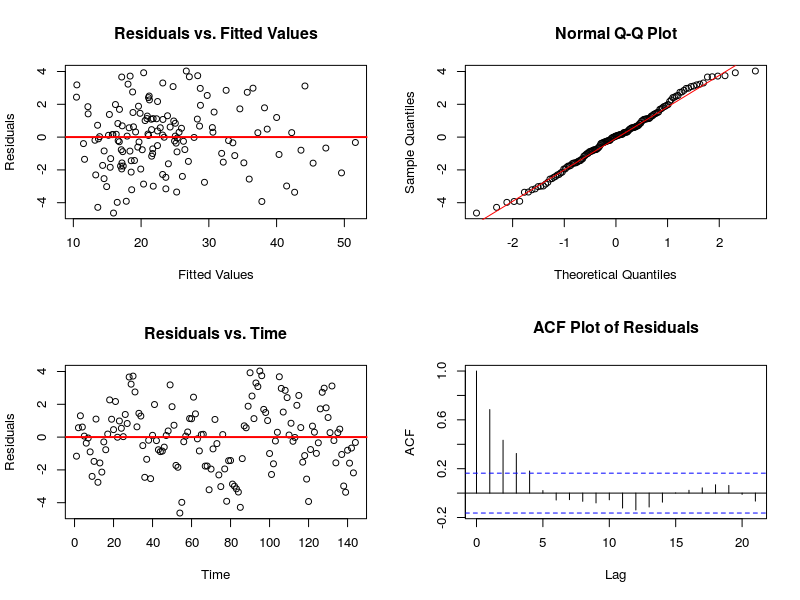
\includegraphics[width=\textwidth]{diag_seas.png}
\caption{Diagnostic plots for quadratic trend and seasonality model.}
\label{diag_seas}
\end{figure}

We can see from the first plot that there seems to be a higher density of values to the left of the graph, which could be a sign of heteroskedasticity. But no clear "funnel-shape" can be distinguished, so homoskedasticity can be assumed. The QQ-plot indicates that the residuals do not deviate too much from normality. From the sequence plot, we can say that the residuals seem randomly distributed and therefore independent. Finally, the ACF plot shows a main pattern of exponential decay with a little bit of seasonality still. Maybe an AR model could be adequate in this data set.

\color{black}

(c) Compare the fit of the model in (b) to the model in part (a).

\color{blue}
By comparing Figures \ref{quad} and \ref{seas}, we can see that the general trend is captured by the quadratic part of the model, while the seasonal part manages to model the monthly oscillations in price. The fit of the model in (b) is better than that of the model in (a).

An F-test comparing the two models can also be calculated since the two models are nested. With R, we get a significant p-value, meaning that the model with quadratic trend and seasonality leads to a significantly lower SSE, which is better. We have also previously seen that the adjusted R-squared is higher for this second model.

A third option is to calculate for example the AIC for each model. We get $804.1723$ for the quadratic trend model and $628.7243$ for the model with trend and seasonality.

All these results indicate that the model in (b) is more adequate for this exercise. 
\color{black}

(d) Which (if either) of the two models above satisfies the fundamental assumptions of least squares regression?

\color{blue}
From the residual diagnostic plots shown in Figures \ref{diag_quad} and \ref{diag_seas}, we can see that neither model passes the assumption of independent residuals. Indeed, for the model in (a), the ACF plot shows significant correlation and seasonality (with a period of around 6, maybe $2\pi$). The ACF plot for the model in (b) shows an exponential decay, with significant autocorrelation at lags 1, 2, 3 (and maybe 4).

This means that neither of these models will be able to make accurate predictions.
\color{black}

(e) Regardless of your response to (d), use the fitted model from (b) to predict the monthly sales data for the year 2011. Add these predictions and the corresponding 95\% prediction intervals to a time series plot of the raw data.

\color{blue}
In order to predict the monthly sales data for the year 2011, we add these predictions and the corresponding 95\% prediction intervals to a time series plot of the raw data using the code below:

\begin{Verbatim}[frame=single]
# Prediction of sales data 
t.new <- seq(2011,2012,length=13)[1:12]
t2.new <- t.new^2
# Introducing the seasonal value for forecasting
month.new <- factor(1:12) 

# Putting the values for forecasting into a dataframe
new <- data.frame(t=t.new, t2=t2.new, month=month.new)
# Computing the prediction as well as prediction interval 
pred <- predict.lm(seas, new, interval='prediction') 

# Plotting the data
plot(sales, xlim=c(1999,2012), ylim=c(0, 65), ylab='Sales',
            main='Sales prediction for 2011')

# Adding a vertical line at the point where prediction starts
abline(v=2011, col='blue', lty=2) 
# Plotting the predict
lines(pred[,1]~t.new, type='l', col='red')
# Plotting lower limit of the prediction interval
lines(pred[,2]~t.new, col='green') 
# Plotting upper limit of the  prediction interval
lines(pred[,3]~t.new, col='green') 
\end{Verbatim}

This produces the plot shown in Figure \ref{pred2011}, where the prediction is in red, and the $95\%$ confidence interval is shown in green. The model seems to do a good job at this prediction. It would be interesting to overlap the actual data for the year 2011 in order to assess how good the prediction was, especially considering our response for (d).

\begin{figure}[!ht]
\centering
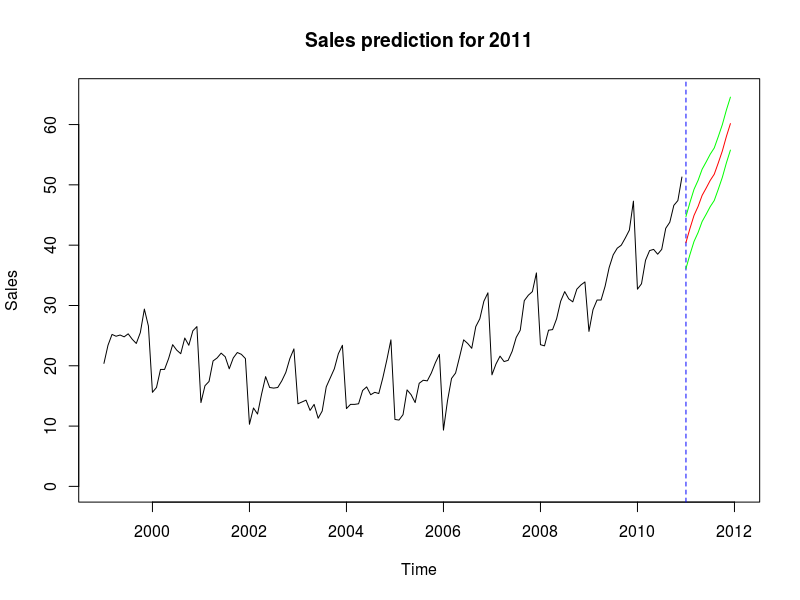
\includegraphics[width=\textwidth]{pred2011.png}
\caption{Prediction and 95\% confidence interval for sales in 2011.}
\label{pred2011}
\end{figure}

\color{black}

\end{document}
